%\section{Estruta da tese e   Etapas da Resolução do Problema}
%
%1. Analisar conjunto de dados. Ver nr de contratos, ver nr de procedimentos e nr de tipo de contratos, etc
%
%2. Categorizar as flags de acordo com a facilidade de implementação e valor
%
%3. Focar, numa fase inicial, num conjunto de contratos. Selecionaram-se apenas ajustes diretos e contratos públicos referentes a CPV's que dizem respeito a %serviços de consultoria de IT - 72

%4. Contruiu-se a primeira flag que compara preço base com preço contratual 
%
%5. Construi-se função que verifica se os precos contratuais dentro dos ajustes diretos caem dentro de um intervalo em torno do preco base
%
%6. Nesta mesma função, inclui-se a presença de um parametro de racio para comparar com precobase/precocontratual. Nos casos em que este quociente é mt alto vai ser verificado se ha ou nao presenca de vários lotes no contrato
%
%7. Construcao de uma funcao que vai analisar ajustes diretos. Priemiro verifica quais os ids dos contratos q ultrapassam o valor maximo permitido por lei q é 20k€. Se ultrapssar dispara a flag. Se num ajuste direto nao houver fundamentação é disparada a flag tambem
%
%8. Os ajustes diretos foram ordenados por ordem crescente de nt de celebracao. Comparou-se o nr de ajustes diretos celebrados com o nt de ajustes suspeitos, calculou-se o racio entre os 2. 
%
%9. No caso dos concursos publicos : qnd o preco base é mt maior que o preco contratual verificar se existem varios id's associados a um mesmo nr de anuncio, somar os preços base e contratual e verificar se o rácio ainda é muito grande

%10. Atribuiu-se um valor de flag contínuo (entre 0 e 1) ao contratos públicos onde é disparada um flag

%11. Contruíu-se uma função que dispara um flag caso o valor do prazo de candidatura de um concurso público seja inferior a 6 dias




\section{Estágio na FORCERA}

%A FORCERA é uma empresa criada em 2021, sediada na região Centro e, embora o seu método de colaboração seja maioritariamente o trabalho remoto, disponibiliza escritório em Lisboa para os seus trabalhadores. A FORCERA enquadra o estatuto de microempresa, contabilizando à data menos de 10 trabalhadores efetivos. Ciente da crescente necessidade dos órgãos públicos em obter maior eficiência, visibilidade e inteligência sobre os seus processos organizacionais, atua ao nível na inovação, sustentabilidade e tecnologia com foco na Administração Pública. Em sintonia com os decisores e respetivas equipas, são identificados os desafios, delineados os objetivos a fim de facilitar o cumprimento das metas estabelecidas. Em paralelo, tem como objetivo construir o expertise tecnológico para o desenvolvimento de novas soluções digitais que facilitem a implementação das estratégias definidas. 


O presente relatório resulta de uma estágio curricular na empresa FORCERA. A FORCERA é uma empresa tecnológica com foco na inovação e sustentabilidade da Administração Pública. Percebendo a crescente necessidade dos órgãos públicos em obter maior eficiência, inteligência e sustentabilidade sobre os seus processos organizacionais e com base na engenharia de software, analítica avançada e inteligência artificial, a empresa dedica-se à produção de soluções inovadoras em diferentes áreas de atuação como finanças, smart cities, ou energia. 
Com escritórios e centro de atividades estabelecido em Lisboa, a FORCERA possui um \textit{track record} de projetos de desenvolvimento e investigação, em parceria com diversas entidades e organizações públicas da Europa Central.

\begin{figure}[H]
	\centering
	
\includegraphics[width=0.7\textwidth]{imagens/forcera.png}
	\caption{Presença da FORCERA na Europeu}
	\label{fig:forcera}
\end{figure}


Dando primazia a iniciativas inovadoras e ambiciosas, a FORCERA distingue-se dentro do setor público através de projetos com clientes de referência como a Câmara Municipal de Lisboa ou com organizações de ação e impacto social como a Better Future. A FORCERA conta com um portfólio de clientes nacionais e internacionais recorrentes (notavelmente a PortX, uma startup FinTech sediada em Londres), e destaca-se por dar respostas a desafios emergentes em diferentes vertentes de sustentabilidade (ambiental, social, energética, financeira, entre outras). Como prova disso, destacam-se os projetos em consórcios europeus como o DigiPrime, que consistiu na criação de uma plataforma de circularidade para equipamentos digitais na Administração Pública, ou o SoTecIn Factory, onde foi desenvolvido o sistema DATA2FORK que permite às organizações públicas obter um scan completo de sustentabilidade ambiental referente a todos os serviços de catering de refeições em espaços públicos.

De salientar que, para lá do enorme expertise tecnológico baseado em várias décadas de experiência acumulada no desenvolvimento de soluções digitais que facilitam a implementação de estratégias organizacionais, a FORCERA aposta muito do seu valor acrescentado através do aspeto consultivo dos serviços prestados. A sua equipa multidisciplinar, composta por programadores, gestores de projeto, consultores, investigadores, apoia a expansão do know-how dos parceiros através da cocriação de estratégias digitais, capacitação, oportunidades de financiamento, ferramentas de apoio, networking e matchmaking e acompanhamento contínuo e incondicional ao longo das várias etapas do projeto.



\section{Fraude e Corrupção na Contratação Pública}


\begin{figure}[H]
	\centering
	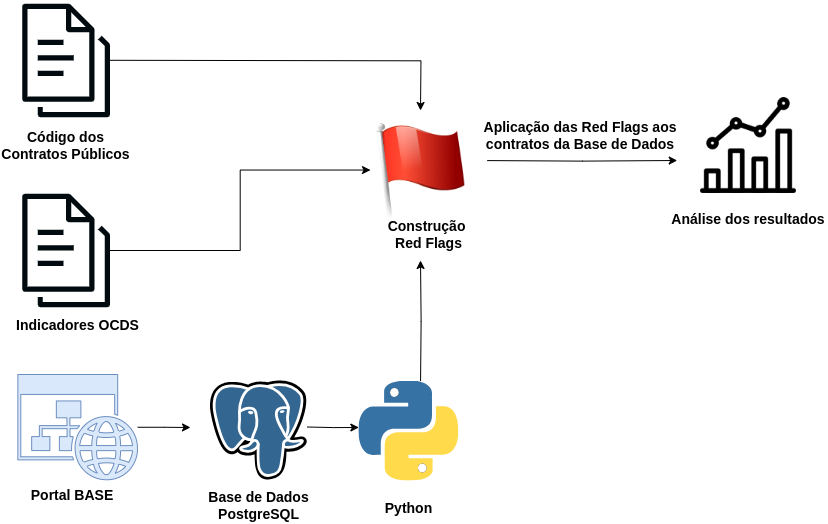
\includegraphics[width=0.85\textwidth]{imagens/processo_tese.png}
	\caption{}
	\label{}
\end{figure}





\section{Organização da tese}

Este relatório encontra-se organizado da seguinte forma: 

\textbf{Capítulo 1 - Introdução:}

\textbf{Capítulo 2 - Contratação Pública em Portugal:}

\textbf{Capítulo 3 - Análise da Base de Dados:}

\textbf{Capítulo 4 - Noções Matemáticas:}

\textbf{Capítulo 5 - Aplicação de \textit{Red Flags}:}

\textbf{Capítulo 6 - Processo de Automação:}

\textbf{Capítulo 7 - Conclusão e Trabalho Futuro:}

